El sistema de adquisición de datos para detectores de muones basa su funcionalidad en un enlace de datos físicos ente una FPGA y una interfaz de lectura ASD, a través de la cual la interfaz emite pulsos digitales mediante emisores LVDS internos y  la FPGA recibe los pulsos con un receptor interno. Este apéndice detalla cómo conectar dispositivos que utilicen interfaces LVDS en cualquier tipo de proyecto, entendiendo los protocolos y requerimientos básicos necesarios para lograrlo.

\section{Acerca del estándar LVDS}	
	LVDS (Low Voltage Differential Signaling) \cite{1996IEEESociety} es un enlace de datos de capa física, útiles en aplicaciones que requieran principalmente conservar la integridad de los datos, mantener bajo ruido en el medio de transmisión, o cuando el emisor y receptor se encuentran demasiado lejos el uno del otro.
	
	Las interfaces LVDS pueden controlar señales en el rango de los 2V a 5V, con una alta velocidad de transferencia de hasta 500Mbps en un solo par diferencial preservando la integridad de la señal a transmitir y manteniendo una buena inmunidad al ruido y a interferencia por campos electromagnéticos Se caracterizan por ser económicas, de bajo consumo de potencia, pequeñas y de una implementación simple.

	Las interfaces LVDS transfieren datos a través de una linea de par trenzado en la que los voltajes de cada cable tienen opuesta amplitud de voltaje. Estas señales son montadas sobre un nivel de voltaje continuo típicamente de 1,2V y poseen tan solo 400mV de diferencia de voltaje ente ambos cables, como se representa en la Figura \ref{fig:lvds-signal}. Esta Figura ilustra una señal LVDS y la compara desde dos perspectivas: en el costado superior se ilustra la señal diferencial interpretándola como un par de terminales independientes, mientras que en costado inferior se ilustra como una señal diferencial, restando los niveles de voltaje de ambas señales. En la imagen, V$_{idth}$ (Input Differential Threshold Voltage) corresponde al nivel de voltaje necesario para que un receptor capte la señal LVDS,  V$_{ob}$ corresponde al cable con potencial de voltaje positivo,  V$_{oa}$ corresponde al cable de potencial negativo y  V$_{od}$ representa la diferencia de voltaje final entre el par de cables.
	
	\begin{figure}[ht]
		\centering
		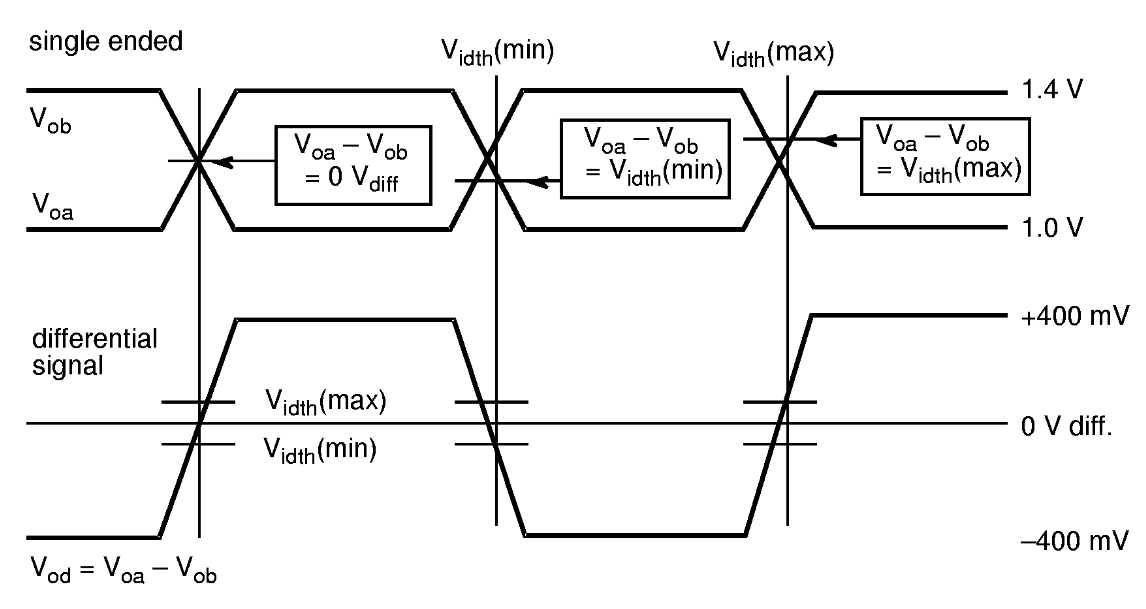
\includegraphics[scale=0.4]{lvds-signal.png}
		\caption{Comparación de una señal diferencial interpretándola como terminales independientes y como terminales diferenciales.}
		\label{fig:lvds-signal}
	\end{figure}
	
	La implementación de una linea de datos LVDS requiere un emisor, una linea de transmisión, una resistencia de 100$\Omega$ y un receptor, como se observa en la Figura \ref{fig:lvds-setup}. La resistencia de 100$\Omega$ se debe a la impedancia propia de la linea de transmisión (50$\Omega$) de cada cable respecto a tierra, junto a una linea de transmisión simétrica se obtiene un medio de comunicación que mantiene la adaptación de impedancia y la integridad de la señal enviada. Las interfaces diferenciales solamente emiten y reciben la diferencia entre los dos cables que componen la linea de transmisión, eliminando el ruido de modo común en la señal de voltaje asociado al potencial eléctrico entre tierra, emisor y receptor, sumado al ruido propio infiltrado en la linea de transmisión.
	
	
	\begin{figure}[ht]
		\centering
		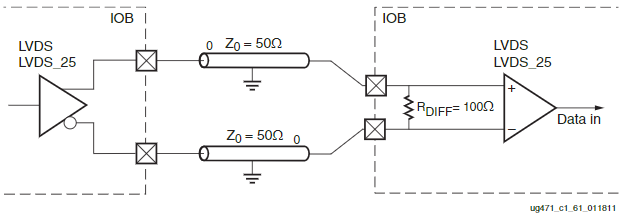
\includegraphics[scale=0.8]{lvds-setup.png}
		\caption{Conexión entre un emisor y receptor LVDS, ubicados a la izquierda y derecha de la imagen respectivamente\cite{Xilinx7UG471}.}
		\label{fig:lvds-setup}
	\end{figure}


\section{Interconexión LVDS para hardware Xilinx 7 Series}

	La familia de FPGAS Xilinx 7 Series\cite{Xilinx20147Guide} es capaz tanto deemitir como recepcionar señales LVDS e incluye la opción de habilitar una resistencia de 100$\Omega$ en caso de que el circuito conectado no cuente con una. Además, esta familia de FPGAs cuenta con dos tipos de estándares LVDS\cite{Xilinx2011Artix-7Characteristics}: el LVDS común, que requiere una fuente de alimentación de 1.8V y se encuentra disponible en los bancos HP (High Performance) de la FPGA, y el estándar LVDS\_25, el cual necesita una fuente de voltaje de 2,5V para alimentar sus bancos de puertos de tipo HR (High Rank). Usar cualquiera de estos dos estándares con su correcta fuente de voltaje permite habilitar o deshabilitar la resistencia interna. De lo contrario, en el caso de usar un voltaje diferente al especificado en el estándar, se debe mantener la resistencia interna desactivada\cite{Xilinx7Banks}.
	
	En particular, la FPGA Artix 7 y la Zynq 7000 tienen solamente bancos HR \cite{Xilinx2011Artix-7Characteristics}, por lo que solo está disponible el estándar LVDS\_25. Contradictoriamente, las tarjetas Trenz utilizadas en esta memoria de titulación solo cuentan con fuentes de 1,8V, 3,3V y 5V, lo que implica que para habilitar la resistencia interna en las FPGAs se debe utilizar una fuente de voltaje externa de 2,5V

\section{Descripción de hardware para utilización de puertos LVDS}

	Para operar correctamente utilizando puertos LVDS en la familia de FPGAs Xilinx 7 Series es necesario declarar los puertos y el estándar seleccionado en el archivo de \textit{constraints} XDC. Por ejemplo para utilizar el par diferencial B16\_L22\_P (positivo) y B16\_L22\_N (negativo) ubicados respectivamente en los puertos E22 y D22 de una FPGA, se declararían las siguientes lineas:

\begin{lstlisting}[language=bash, frame=single, basicstyle=\tiny]
set_property -dict {PACKAGE_PIN E22 IOSTANDARD LVDS_25} [get_ports B16_L22_P];
set_property -dict {PACKAGE_PIN D22 IOSTANDARD LVDS_25} [get_ports B16_L22_N];
\end{lstlisting}


	Finalmente, para poder utilizar correctamente el par diferencial, es necesario utilizar un \textit{IO Buffer} instanciándolo en el hardware descrito. Estos buffers permiten convertir la señal diferencial a una de un solo terminal o viceversa. Por ejemplo, para usar un par diferencial según el estándar LVDS\_25 habilitando la resistencia interna del puerto, bastaría con declarar un IBUFDS (Input Buffer for Differential Singal)\cite{Xilinx2012XilinxDesigns} como se indica a continuación:
	

\begin{lstlisting}[language=Verilog, frame=single, basicstyle=\tiny]
// IBUFDS: Differential Input Buffer - Verilog
// 7 Series
// Xilinx HDL Libraries Guide, version 13.4
IBUFDS #(
    .DIFF_TERM("TRUE"), // Differential Termination (TRUE or FALSE)
    .IBUF_LOW_PWR("FALSE"), // Low power="TRUE", Highest performance="FALSE"
    .IOSTANDARD("LVDS_25") // Specify the input I/O standard (LVDS or LVDS_25)
    ) IBUFDS_LVDS_25 (
    .O(lvds_output), // Buffer output
    .I(B16_L22_P), // Diff_p buffer input (connect directly to top-level port)
    .IB(B16_L22_N) // Diff_n buffer input (connect directly to top-level port)
);
// End of IBUFDS_inst instantiation
\end{lstlisting}

Siguiendo estos pasos, el receptor LVDS queda correctamente configurado. Para utilizar el receptor LVDS basta con conectar las respectivas señales diferenciales en los puertos correspondientes declarados en el diseño, utilizando siempre un cable de par trenzado simétrico con una impedencia de 50$\Omega$.